\subsection{Промежуточные  представления  программы:  абстрактное  синтаксическое  дерево;  последовательность трехадресных инструкций. Базовые блоки и граф потока управления.}

\textbf{Промежуточное представление программы} (Intermediate Representation, IR) --- форма представления программы, ориентированная на удобство дальнейшей обработки компилятором.

Различают следующие IR:
\begin{itemize}
    \item HIR (высокий уровень) --- абстрактное синтаксическое дерево(АСД) --- конечное помеченное ориентированное дерево, в котором внутренние вершины сопоставлены (помечены) с операторами языка программирования, а листья --- с соответствующими операндами. По сути результат парсинга программы на языке программирования, по АСД можно однозначно восстановить программу, по остальным уже нельзя.
    \item MIR (средний уровень) --- включает в себя:
    \begin{enumerate}
        \item Инструкции
        \item[--] присваивание: \texttt{x <- op y z; x <- op y; x <- y;}
        \texttt{x[i] <- y; x <- y[i];},
        \item[--] переходы: \texttt{goto L; ifTrue x goto L; ifFalse x goto L;}
        \item[--] дополнительное: \texttt{param x; call x n; return y;}
        \item таблицу символов,
        \item[--] переменные, их имена в программе и атрибуты, такие как область видимости, тип, для имен функций - число параметров, и т. п.
    \end{enumerate}
    \item LIR (низкий уровень) --- фактически машинные инструкции --- используется для машинно-зависимых задач, например, распределение регистров и выбор подходящих команд.
\end{itemize}

\textbf{Базовые блоки и граф потока управления}

\textbf{Базовым блоком} (ББ или линейным участком) называется последовательность следующих одна за другой инструкций MIR, обладающая следующими свойствами:
\begin{itemize}
    \item Поток управления может входить в базовый блок только через его первую инструкцию (т.е. в программе нет переходов в середину базового блока),
    \item Поток управления покидает базовый блок без останова или ветвления, кроме, возможно, последней инструкции базового блока.
\end{itemize}

Грубо говоря, \textit{базовый блок} содержит инструкции, которые будут выполнены (или не выполнены) обязательно все вместе, независимо ни от чего. Поэтому он базовый.

Чтобы выделить базовые блоки, достаточно найти все их начала (НББ):
\begin{itemize}
    \item первая инструкция программы
    \item инструкция, на которой есть метка
    \item следующая инструкция после перехода
\end{itemize}

\textit{Граф потока управления} (ГПУ) --- граф, обладающий следующими свойствами:
\begin{itemize}
    \item Вершины --- базовые блоки.
    \item Дуга соединяет выход одного блока со входом другого, если второй блок может выполняться сразу следом за первым.
    
    Если последняя инструкция базового блока --- условный переход, то из этого блока будут выходить две дуги. 
    
    Если первая инструкция базового блока имеет метку, то в этот блок будут входить дуги из всех базовых блоков, у которых последняя инструкция --- переход на эту метку.
\end{itemize}

Чтобы построить ГПУ, надо 
\begin{enumerate}
    \item выделить базовые блоки;
    \item Провести дугу из блока туда, куда может пойти управление после этого блока. Определяется по последней инструкции: 
    \item[--] либо просто следующий блок
    \item[--] либо это безусловный переход - туда где метка этого перехода
    \item[--] либо и туда и туда, если это условный переход
\end{enumerate}

Пример ГПУ:

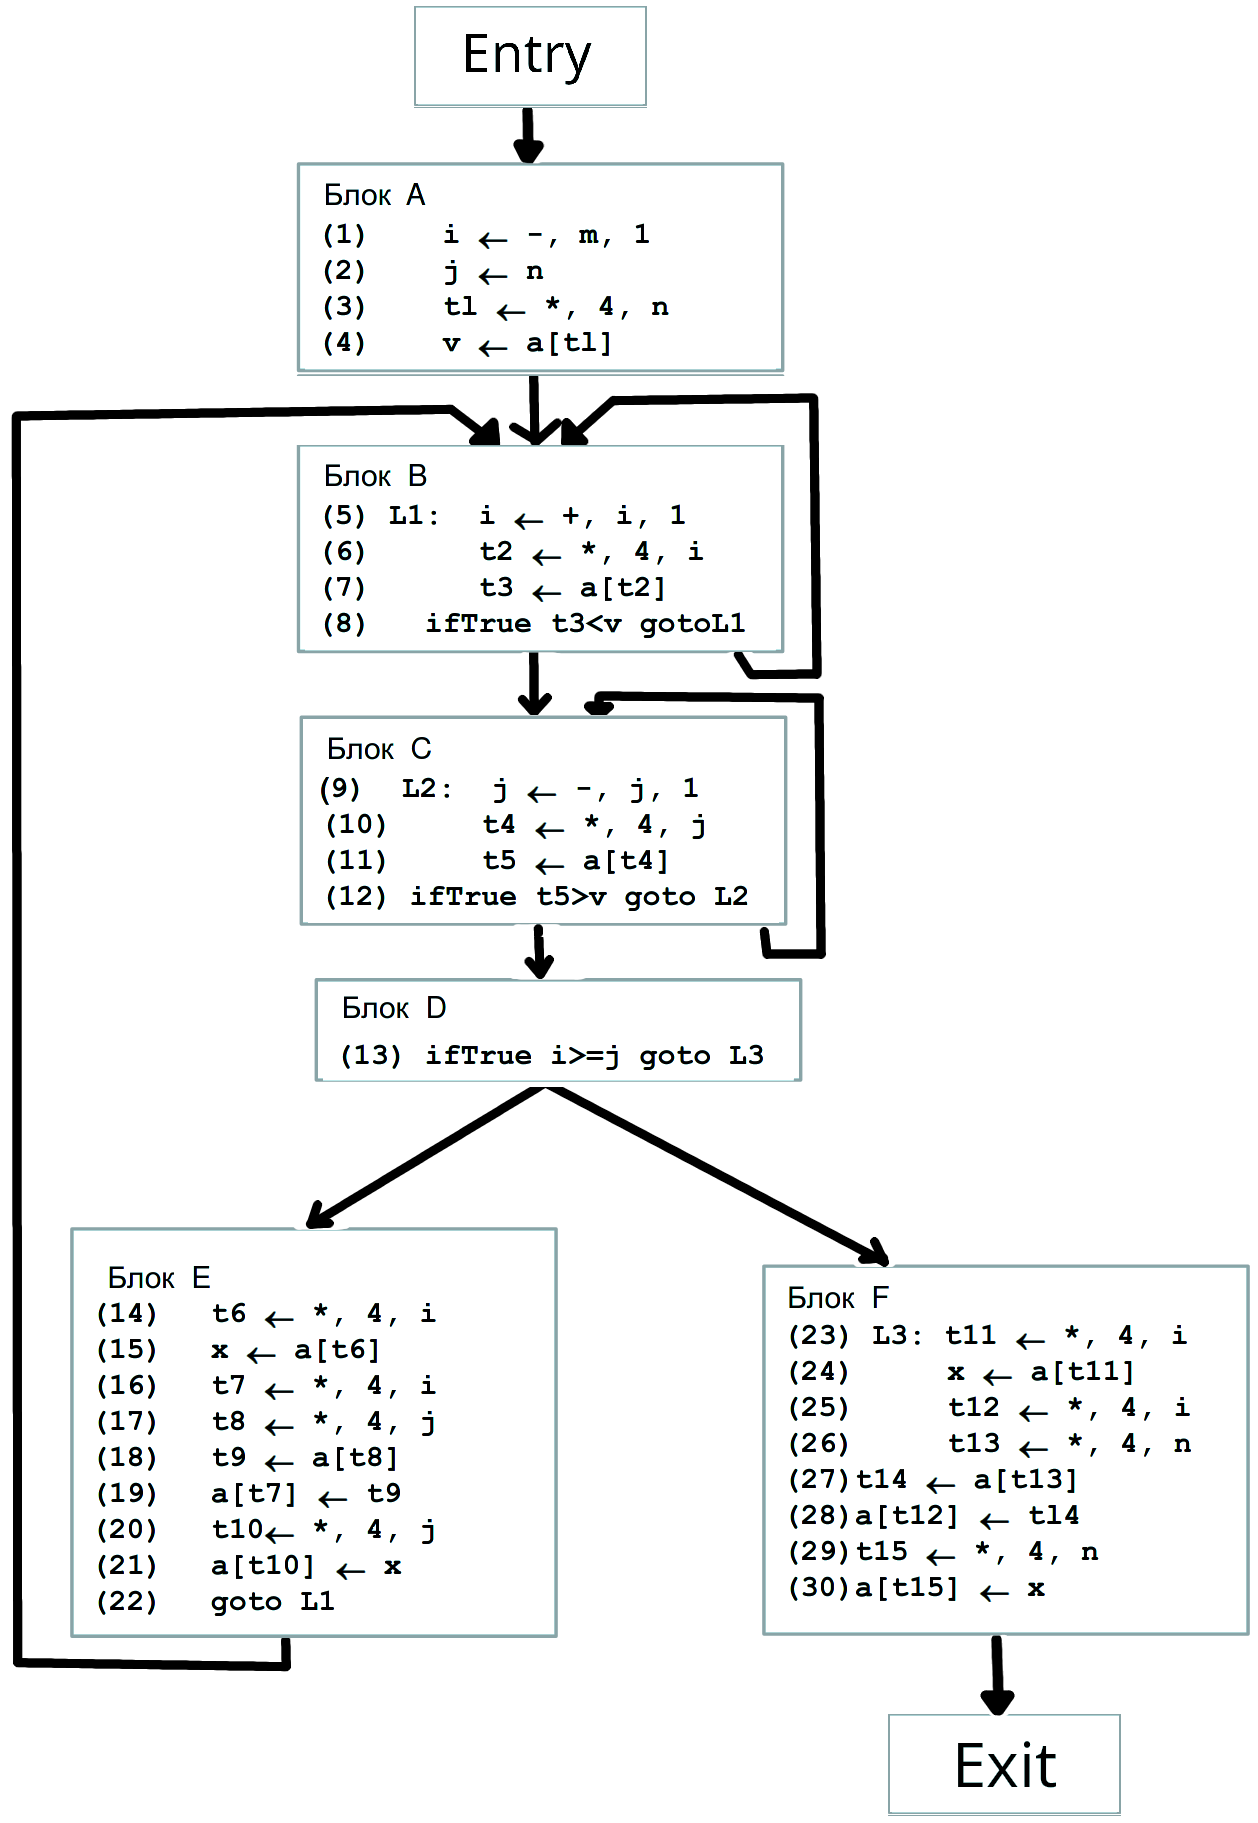
\includegraphics[width=\columnwidth]{pics/cfg.png}

% -------- source --------
\bigbreak
[\cite[slide 7-28]{ssg}]